Our final issue is the cross section of DM annihilating into SM particles (fig. \ref{pic_annihilation}). So as for $B_s\rightarrow \mu\mu$, all model parameters are taken into
account
\begin{align}
 \left(m_\chi, M_l, M_q, g^l_2\right)
\end{align}
We assume $\chi^0$ to be a Majorana fermion which already implies that its s-wave cross section into a fermion pair is helicity suppressed and 
thus the leading contribution is p-wave \cite{1307.8120}. This can be explained as follows considering charge ($C$) and parity ($P$) symmetries.
The respective transformations for a fermion/antifermion state is $C=(-1)^{L+S},\,P=(-1)^{L+1}$ with the total spin $S$ and the total orbital angular
momentum $L$. 
In the Majorana case $C=+1$. s-wave further means $S=0$ and hence $P=-1$. The $\bar f f$ state shall be able to reproduce the same $J=|L\pm S|$ 
which only has $S=0$ when the fermion and the antifermion are different Weyl spinors, i.e. a left handed fermion and a left handed antifermion.
In chiral models like ours, in the limit of zero quark mass, we have $S=1$ giving $C=(-1)^{L+1},\,P=(-1)^{L+1}$ and therefore $C$ and $P$ are not 
conserved for any $L$. So for s-wave annihilation a helicity flip, as for the anomalous magnetic moment of the muon, proportional to $m_f$ is 
required. Despite the fact that the muon is very light, it has an anticipated large coupling, above unity. The top quarks coupling is of order unity
but also has a large mass. So we expect leading contributions for the annihilation from these two particles shaping the final state.
\begin{figure}[t]
 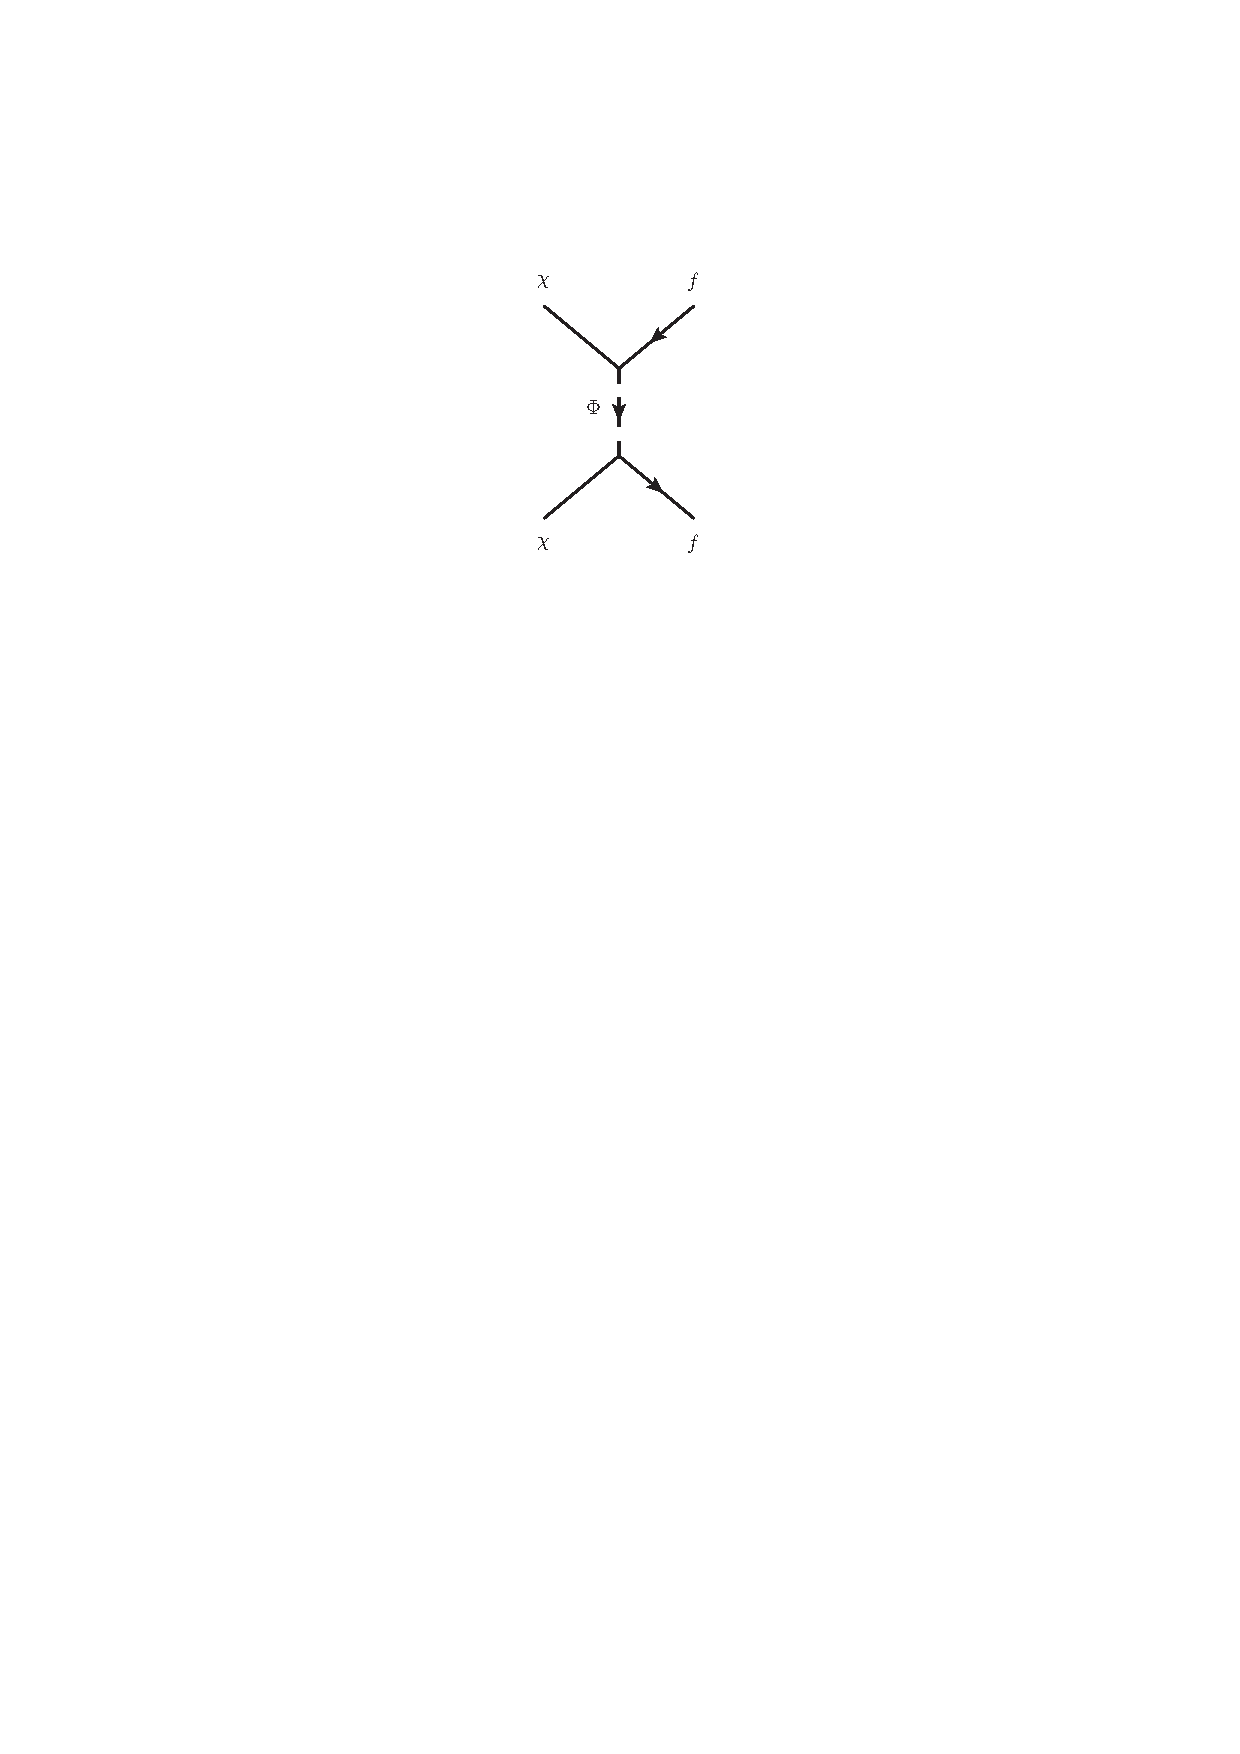
\includegraphics[width=1\textwidth]{../pics/ann.pdf}
 \caption{Annihilation process.}
 \label{pic_annihilation}
\end{figure}
% $VV$ annihilation (9207234), wino RD from other su2-states (0913-main)
% \begin{align}
%  \langle \sigma v \rangle^\text{D} \left(\bar \chi \chi \rightarrow \bar f f\right) = \frac{N_c g_f^4 m^2}{32\pi^2\left(M_l^2 + m^2\right)^2}
% \end{align}
The thermally averaged annihilation cross section into fermions is independent of the representations \cite{1503.01500}
\begin{align}
 \langle \sigma v \rangle \left(\bar \chi^0 \chi^0 \rightarrow \bar f f\right) = \frac{N_c g_f^4}{32\pi m_\chi^2\left(1+x_f\right)^2} \left(\frac{m_f^2}{m_\chi^2} + \frac{2\left(1+x_f\right)^2}{3\left(1+x_f\right)^2} v^2\right)  .
\end{align}
For the triplet there is an additional tree level decay into $W$-bosons which is, in some region, roughly as dominant as the decay into muons. 
For bosons there is no helicity or velocity suppression at leading order. The cross section reads\cite{1401.6212}
\begin{align}
 \langle \sigma v \rangle \left(\bar \chi^0 \chi^0 \rightarrow W^+W^-\right) = \frac{8\pi \alpha_2^2}{m_\chi^2} \frac{(1-w)^{\sfrac32}}{(2-w)^2}.
\end{align}
No co-annihilations are considered here for assumed non-degeneracy of $m_\chi$ and $M_{l,q}$. The velocity $v$ at the time when DM decoupled is
estimated as $v\approx 0.3$. 
%Nowadays $2\rightarrow3$ processes as $\bar \chi \chi \rightarrow \bar f f V$ might dominate with lower velocities 
%$v\approx 10^{-3}$, interesting for indirect detection \cite{1207.1431}. 